% ==============================================================
% 10_ppg_extension_presentation.tex
% "Beyond League Position: Points, Points-Per-Game, and the
%  Search for the Right Outcome Measure"
% Supplementary extension deck to 09_presentation.tex, covering the
% extensions/ folder analysis (Model A -> H Position -> H Points ->
% H PPG evolution, standardised effects, inflation robustness,
% PPG residuals, and the SPAL data correction).
% Beamer / Metropolis — compile with: xelatex deliverables/presentation/10_ppg_extension_presentation.tex
% (run from project root so \graphicspath resolves)
% ==============================================================
\documentclass[aspectratio=1610,10pt]{beamer}

% ── Metropolis theme ──────────────────────────────────────────
\usetheme[progressbar=frametitle, block=fill, numbering=fraction]{metropolis}

% ── xelatex font setup ───────────────────────────────────────
\usepackage{fontspec}
\usepackage{microtype}

% ── Core packages ─────────────────────────────────────────────
\usepackage{graphicx}
\usepackage{booktabs}
\usepackage{colortbl}
\usepackage{xcolor}
\usepackage{tikz}
\usepackage{array}
\usepackage{amsmath}
\usepackage{url}
\usepackage{calc}

% ── Image path (compile from project root) ────────────────────
\graphicspath{{extensions/outputs/}{outputs/}}

% ── Project colour palette (identical to 09_presentation.tex) ──
\definecolor{NavyBlue}{HTML}{1A2A4A}
\definecolor{PitchGold}{HTML}{F5A623}
\definecolor{AlertRed}{HTML}{C0392B}
\definecolor{GrassGreen}{HTML}{196F3D}
\definecolor{SteelBlue}{HTML}{2C3E73}
\definecolor{SlateGrey}{HTML}{566573}
\definecolor{RowA}{HTML}{EBF5FB}
\definecolor{RowB}{HTML}{FEF9E7}
\definecolor{LightRed}{HTML}{FDEDEC}

% ── Metropolis colour overrides ───────────────────────────────
\setbeamercolor{normal text}{fg=NavyBlue, bg=white}
\setbeamercolor{frametitle}{bg=NavyBlue, fg=white}
\setbeamercolor{title separator}{fg=PitchGold}
\setbeamercolor{progress bar}{fg=PitchGold, bg=NavyBlue!25}
\setbeamercolor{progress bar in section page}{fg=PitchGold, bg=NavyBlue!25}
\setbeamercolor{alerted text}{fg=AlertRed}
\setbeamercolor{example text}{fg=GrassGreen}
\setbeamercolor{block title}{bg=NavyBlue!12, fg=NavyBlue}
\setbeamercolor{block body}{bg=NavyBlue!5, fg=NavyBlue}
\setbeamercolor{block title alerted}{bg=AlertRed!12, fg=AlertRed}
\setbeamercolor{block body alerted}{bg=AlertRed!5}
\setbeamercolor{block title example}{bg=GrassGreen!12, fg=GrassGreen}
\setbeamercolor{block body example}{bg=GrassGreen!5}

\metroset{titleformat=smallcaps}

% ── TU Dortmund logo (conditional on file presence) ───────────
\IfFileExists{tu-do-logo.pdf}{%
  \titlegraphic{\hfill\includegraphics[height=1.0cm]{tu-do-logo.pdf}}%
}{\titlegraphic{}\logo{}}

% ── Presentation metadata ─────────────────────────────────────
\title{Beyond League Position}
\subtitle{Points, Points-Per-Game, and the Search for the Right Outcome Measure}
\author[Group X]{%
  \texorpdfstring{%
    {\small\textbf{Group X:}\\[0.2em]
    Md Muktadir \quad|\quad Linus Mainka}%
  }{Group X}}
\institute{\small TU Dortmund University
  \textendash{} Department of Statistics}
\date{\small Summer Semester 2026 \quad|\quad
  Supplementary Extension Analysis}

% ── Callout box commands (identical to 09_presentation.tex) ────
\newcommand{\findingbox}[1]{%
  \begin{tikzpicture}
    \node[fill=PitchGold!18, draw=PitchGold, line width=0.9pt,
          rounded corners=4pt, inner sep=9pt,
          text width=\linewidth-10pt]%
      {\small\bfseries\color{NavyBlue}#1};
  \end{tikzpicture}}

\newcommand{\alertbox}[1]{%
  \begin{tikzpicture}
    \node[fill=AlertRed!10, draw=AlertRed, line width=0.9pt,
          rounded corners=4pt, inner sep=9pt,
          text width=\linewidth-10pt]%
      {\small\bfseries\color{AlertRed}#1};
  \end{tikzpicture}}

\newcommand{\statpanel}[2]{%
  \begin{tikzpicture}
    \node[fill=NavyBlue!7, draw=NavyBlue!25, line width=0.6pt,
          rounded corners=4pt, inner sep=9pt,
          text width=\linewidth-10pt, align=center]%
      {{\large\bfseries\color{NavyBlue}#1}\par\smallskip
       {\footnotesize\color{SlateGrey}#2}};
  \end{tikzpicture}}

\newcommand{\duallabel}[2]{%
  \begin{tikzpicture}
    \node[fill=RowA, draw=SteelBlue!30, line width=0.5pt,
          rounded corners=3pt, inner sep=8pt,
          text width=\linewidth-10pt]%
      {{\footnotesize\textbf{\color{SteelBlue}Statistical:}~#1}%
       \par\smallskip
       {\footnotesize\textbf{\color{GrassGreen}Plain English:}~#2}};
  \end{tikzpicture}}

% ─────────────────────────────────────────────────────────────
\begin{document}

% ══════════════════════════════════════════════════════════════
% SLIDE 1 — Title
% ══════════════════════════════════════════════════════════════
\maketitle

% ══════════════════════════════════════════════════════════════
% SLIDE 2 — Motivation
% ══════════════════════════════════════════════════════════════
\begin{frame}[shrink=8]{Why Look Beyond League Position?}
  \vspace{2pt}
  {\normalsize\color{NavyBlue}%
   \textbf{Follow-up question:} does the money--success finding survive if
   we change how we measure ``success'' --- or is it an artifact of using
   final league position?}
  \vspace{8pt}

  \begin{columns}[T]
    \begin{column}{0.54\textwidth}
      \textbf{Two problems with the outcomes used so far:}
      \begin{itemize}\setlength\itemsep{6pt}
        \item \textbf{League position} is ordinal and bounded (1--20):
              easy to compare across leagues, but blind to \emph{margin}
              --- finishing 1st by 1 point looks identical to finishing
              1st by 20.
        \item \textbf{Total points} are \emph{not} directly comparable
              across leagues: the Bundesliga plays 34 matches per season,
              the other four leagues play 38. A team on 70 points after
              34 matches is dominating far more than one on 70 points
              after 38.
      \end{itemize}
    \end{column}
    \begin{column}{0.42\textwidth}
      \vspace{4pt}
      \findingbox{The professor's suggestion: normalise by matches
        played --- \textbf{Points Per Game (PPG)} --- a genuinely
        cross-league-comparable outcome.}
      \vspace{8pt}
      {\small\color{SlateGrey}
        This deck re-runs the full analysis three times --- Position,
        Points, PPG --- to see whether the core finding changes.}
    \end{column}
  \end{columns}
\end{frame}

% ══════════════════════════════════════════════════════════════
% SLIDE 3 — Data Correction Footnote
% ══════════════════════════════════════════════════════════════
\begin{frame}[shrink=8]{One Correction Before Extending the Model}
  \begin{columns}[T]
    \begin{column}{0.52\textwidth}
      \textbf{What we found:} SPAL (Serie A, 2017--18) never matched a
      name during the original ESPN/Transfermarkt merge, leaving its
      \texttt{Market\_Value} and \texttt{Financial\_Rank} missing ---
      the \textbf{only} gap in 976 team-seasons.
      \vspace{6pt}

      \textbf{What we did:} inserted SPAL's true 2017--18 squad value
      (\texteuro{}63.55M, Transfermarkt) and recomputed Financial Rank
      for that one league-season.
      \vspace{6pt}

      \textbf{Independent confirmation:} SPAL lands at \textbf{FR\,16}
      --- exactly the numbering gap that already existed in the
      untouched data (ranks jumped 15\,$\to$\,17 before the fix).
    \end{column}
    \begin{column}{0.44\textwidth}
      \vspace{2pt}
      \alertbox{Before the fix, the inflation-adjustment check
        (Slide~9) showed \textbf{4 apparent rank changes}. All four
        were this one data gap, not inflation. After the fix:
        \textbf{0}.}
      \vspace{8pt}
      {\footnotesize\color{SlateGrey}
        Every result in this deck --- and the corresponding update to
        the main presentation --- uses the corrected dataset
        (\texttt{master\_dataset\_corrected.csv}).}
    \end{column}
  \end{columns}
\end{frame}

% ══════════════════════════════════════════════════════════════
% SLIDE 4 — Four Specifications, One Predictor
% ══════════════════════════════════════════════════════════════
\begin{frame}[shrink=8]{Four Specifications, One Predictor: Financial Rank}
  \vspace{4pt}
  {\small
  \begingroup\setlength{\tabcolsep}{4pt}
  \begin{tabular}{@{}l l r r r r r@{}}
    \toprule
    \rowcolor{NavyBlue!18}
    \color{white}\textbf{Model} &
    \color{white}\textbf{Outcome} &
    \color{white}$R^2$ &
    \color{white}Adj.\,$R^2$ &
    \color{white}\textbf{AIC} &
    \color{white}FR coef. &
    \color{white}FR$^2$ coef. \\
    \midrule
    A: Linear baseline & League Position & 0.661 & 0.660 & 5104.4 & $+0.813$ & --- \\
    \rowcolor{RowA}
    H: Quadratic & League Position & 0.671 & 0.671 & 5075.1 & $+1.231$ & $-0.020$ \\
    H: Quadratic & Total Points & 0.678 & 0.677 & 7234.6 & $-5.047$ & $+0.127$ \\
    \rowcolor{RowB}
    \textbf{H: Quadratic} & \textbf{Points Per Game} & \textbf{0.696} & \textbf{0.695} & \textbf{100.1} & $\mathbf{-0.134}$ & $\mathbf{+0.003}$ \\
    \bottomrule
  \end{tabular}
  \endgroup
  }
  \vspace{10pt}
  \findingbox{Same predictor, four scoring systems. The bottom row ---
    the professor's suggested PPG specification --- achieves the
    \textbf{highest $R^2$ of any model tried in this project}
    ($N = 976$ throughout).}
\end{frame}

% ══════════════════════════════════════════════════════════════
% SLIDE 5 — Four Panels, Side by Side
% ══════════════════════════════════════════════════════════════
\begin{frame}{Four Panels, Side by Side}
  \begin{center}
    
\includegraphics[width=0.92\linewidth,
                     height=0.80\textheight,
                     keepaspectratio]{E2_model_evolution_4panel.png}
  \end{center}
\end{frame}

\begin{frame}[shrink=8]{What the Four Panels Show}
  \findingbox{Every panel shows the same downward-bending curve:
    richer squads (low FR) outperform, poorer squads (high FR)
    underperform, and the gap narrows as FR grows --- diminishing
    returns hold under \textbf{every} outcome measure tested,
    from the simplest linear baseline to points per game.}
\end{frame}

% ══════════════════════════════════════════════════════════════
% SLIDE 6 — Points Per Game: the Fairest Comparison
% ══════════════════════════════════════════════════════════════
\begin{frame}[shrink=8]{Points Per Game: Why It's the Fairest Comparison}
  \begin{columns}[T]
    \begin{column}{0.48\textwidth}
      \begin{block}{Definition}
        {\small
        \[\text{PPG} = \frac{\text{Points}}{\text{Matches Played}}\]
        \vspace{2pt}
        Matches played: \textbf{34} for the Bundesliga,
        \textbf{38} for La Liga, Ligue~1, Premier League, and
        Serie~A.}
      \end{block}
      \vspace{6pt}
      {\small\begin{itemize}\setlength\itemsep{5pt}
        \item Removes the schedule-length distortion baked into raw
              \emph{Points}.
        \item Puts every club, in every league, in every season, on
              the \textbf{same per-match scale}.
      \end{itemize}}
    \end{column}
    \begin{column}{0.48\textwidth}
      {\small
      \begin{tabular}{@{}l r@{}}
        \toprule
        \rowcolor{NavyBlue!18}
        \color{white}\textbf{Outcome} & \color{white}$R^2$ \\
        \midrule
        League Position & 0.671 \\
        \rowcolor{RowA}
        Total Points     & 0.678 \\
        \rowcolor{RowB}
        \textbf{Points Per Game} & \textbf{0.696} \\
        \bottomrule
      \end{tabular}
      }
      \vspace{10pt}
      \findingbox{PPG doesn't just satisfy the professor's request ---
        it produces the \textbf{tightest fit of all three} outcome
        measures.}
    \end{column}
  \end{columns}
\end{frame}

% ══════════════════════════════════════════════════════════════
% SLIDE 7 — Standardised Effect Comparison
% ══════════════════════════════════════════════════════════════
\begin{frame}{Standardised Effect Comparison: Reading the Numbers Correctly}
  \begin{center}
    
\includegraphics[width=0.85\linewidth,
                     height=0.68\textheight,
                     keepaspectratio]{E4b_standardised_effect_comparison.png}
  \end{center}
\end{frame}

\begin{frame}[shrink=8]{Interpreting the Standardised Effect Chart}
  \begin{columns}[T]
    \begin{column}{0.52\textwidth}
      {\small\begin{itemize}\setlength\itemsep{6pt}
        \item Chart shows: predicted change from FR\,1 to FR\,20,
              as a \% of that outcome's \emph{observed range}.
        \item Position models: $\approx$\,81\,\%. Points/PPG models:
              $\approx$\,51--53\,\%.
        \item \textbf{Why the gap?} League position is bounded
              1--20 \emph{by construction} --- almost the entire
              scale is mechanically ``used.'' Points and PPG
              reflect genuine match variation, not a fixed scale.
      \end{itemize}}
    \end{column}
    \begin{column}{0.44\textwidth}
      \vspace{2pt}
      \alertbox{This is \textbf{not} evidence that PPG predicts
        ``less well.'' $R^2$ (Slide~4) is the correct measure of
        fit --- and PPG scores \textbf{highest} there. This chart
        measures something different: how much of the observed
        spread the FR effect spans.}
    \end{column}
  \end{columns}
\end{frame}

% ══════════════════════════════════════════════════════════════
% SLIDE 8 — Coefficient Evolution: the Sign Flip
% ══════════════════════════════════════════════════════════════
\begin{frame}{Coefficient Evolution Across Specifications}
  \begin{center}
    
\includegraphics[width=0.80\linewidth,
                     height=0.68\textheight,
                     keepaspectratio]{E4_coefficient_evolution.png}
  \end{center}
\end{frame}

\begin{frame}[shrink=8]{The Sign Flip Is Definitional, Not a Contradiction}
  \duallabel{The Financial\_Rank coefficient is \textbf{positive} for
    Position ($+0.81$, $+1.23$) and \textbf{negative} for Points and
    PPG ($-5.05$, $-0.13$).}{Higher FR always means a worse outcome
    --- it just points in opposite arithmetic directions depending on
    whether ``worse'' means a bigger position number or a smaller
    points total.}
  \vspace{10pt}
  \findingbox{Whichever way the sign points, the message is
    identical: moving from the richest squad (FR\,1) to the poorest
    (FR\,20) costs a club dearly, on every scale tested.}
\end{frame}

% ══════════════════════════════════════════════════════════════
% SLIDE 9 — Inflation Robustness
% ══════════════════════════════════════════════════════════════
\begin{frame}{Does Financial Rank Itself Survive Ten Years of Inflation?}
  \begin{center}
    
\includegraphics[width=0.92\linewidth,
                     height=0.68\textheight,
                     keepaspectratio]{E3_inflation_validation.png}
  \end{center}
\end{frame}

\begin{frame}[shrink=8]{Why This Matters for Every Model in This Deck}
  \begin{columns}[T]
    \begin{column}{0.50\textwidth}
      {\small\begin{itemize}\setlength\itemsep{6pt}
        \item Average squad value roughly \textbf{doubled} 2015--16
              to 2024--25 (index 0.59\,$\to$\,1.30, 2019--20\,$=$\,1.00).
        \item But \textbf{Financial\_Rank} is a \emph{within-season}
              rank, not a raw euro figure --- dividing every club in
              a league-season by the same constant cannot change
              their relative order.
        \item After the SPAL fix: \textbf{0 genuine rank changes} in
              all 976 team-seasons, confirmed individually in
              \emph{every} one of the five leagues.
      \end{itemize}}
    \end{column}
    \begin{column}{0.44\textwidth}
      \vspace{2pt}
      \findingbox{Every model in this deck --- Position, Points,
        PPG --- is fed the \textbf{same season-stable predictor}.
        Inflation cannot be driving any of these results.}
    \end{column}
  \end{columns}
\end{frame}

% ══════════════════════════════════════════════════════════════
% SLIDE 10 — PPG Residuals: Does Leicester Still Win?
% ══════════════════════════════════════════════════════════════
\begin{frame}{PPG Residuals: Does Leicester Still Win?}
  \begin{center}
    
\includegraphics[width=0.80\linewidth,
                     height=0.78\textheight,
                     keepaspectratio]{E5_ppg_residuals.png}
  \end{center}
\end{frame}

\begin{frame}[shrink=8]{Leicester City 2015--16: Still the Greatest Outlier}
  \begin{columns}[T]
    \begin{column}{0.48\textwidth}
      {\small
      \begin{tabular}{@{}l l@{}}
        \toprule
        \rowcolor{NavyBlue!18}
        \multicolumn{2}{l}{\color{white}\textbf{PPG Model Diagnostics}} \\
        \midrule
        Residual SD          & 0.254 PPG \\
        \rowcolor{RowA}
        $\pm$1.5\,SD threshold & $\pm$0.381 PPG \\
        Overperformers        & 56 teams \\
        \rowcolor{RowA}
        Underperformers        & 71 teams \\
        \bottomrule
      \end{tabular}
      }
    \end{column}
    \begin{column}{0.48\textwidth}
      \vspace{2pt}
      \alertbox{\textbf{Leicester City 2015--16}: residual
        $= +0.923$ PPG --- the single \textbf{largest residual of
        all 976 team-seasons}, rank \#1. Even under the professor's
        preferred specification, Leicester's title remains the
        greatest financial upset in the dataset.}
    \end{column}
  \end{columns}
\end{frame}

% ══════════════════════════════════════════════════════════════
% SLIDE 11 — Two Honest Caveats
% ══════════════════════════════════════════════════════════════
\begin{frame}[shrink=8]{Two Honest Caveats About PPG}
  \vspace{4pt}
  \begin{columns}[T]
    \begin{column}{0.48\textwidth}
      \begin{alertblock}{COVID-Shortened Ligue~1, 2019--20}
        {\small Season stopped after \textbf{27} of the assumed
        38 matches. PPG still divides by 38 (per the original
        specification), so that season's Ligue~1 PPG values are
        biased \textbf{downward} relative to completed seasons.
        Flagged, not corrected.}
      \end{alertblock}
    \end{column}
    \begin{column}{0.48\textwidth}
      \begin{exampleblock}{Ligue~1's 2023--24 Format Change}
        {\small Ligue~1 moved to an 18-club, \textbf{34}-match
        format from 2023--24 onward --- the same 34-vs-38 divisor
        mismatch affects those two seasons.}
      \end{exampleblock}
    \end{column}
  \end{columns}
  \vspace{10pt}
  \duallabel{3 of the 50 league-seasons in the dataset deviate from
    the assumed 38-match schedule (all Ligue~1).}{A handful of
    Ligue~1 PPG values should be read with this caveat in mind ---
    no other league or season is affected.}
\end{frame}

% ══════════════════════════════════════════════════════════════
% SLIDE 12 — Conclusion
% ══════════════════════════════════════════════════════════════
\begin{frame}[shrink=8]{Conclusion: Same Story, Sharper Lens}
  \vspace{2pt}

  \noindent\fcolorbox{NavyBlue!20}{NavyBlue!7}{%
    \parbox{\dimexpr\textwidth-2\fboxrule-2\fboxsep}{%
      {\footnotesize\bfseries\color{NavyBlue}1.\ Financial Rank predicts success under every outcome measure tried.}\\[2pt]
      {\scriptsize\color{SlateGrey}$R^2 = 0.671$ (Position), $0.678$ (Points), $\mathbf{0.696}$ (PPG) --- all $N=976$, all $p<0.001$.}}}
  \vspace{4pt}

  \noindent\fcolorbox{NavyBlue!20}{NavyBlue!7}{%
    \parbox{\dimexpr\textwidth-2\fboxrule-2\fboxsep}{%
      {\footnotesize\bfseries\color{NavyBlue}2.\ PPG is the most defensible outcome measure of the three.}\\[2pt]
      {\scriptsize\color{SlateGrey}The only measure directly comparable across leagues with unequal season lengths --- and it fits best.}}}
  \vspace{4pt}

  \noindent\fcolorbox{AlertRed!50}{AlertRed!8}{%
    \parbox{\dimexpr\textwidth-2\fboxrule-2\fboxsep}{%
      {\footnotesize\bfseries\color{AlertRed}3.\ Leicester City 2015--16 is not an artifact of choosing ``league position.''}\\[2pt]
      {\scriptsize\color{NavyBlue}It is the single largest overperformance under points \textbf{and} under PPG --- the anomaly survives every outcome measure.}}}
  \vspace{4pt}

  \noindent\fcolorbox{NavyBlue!20}{NavyBlue!7}{%
    \parbox{\dimexpr\textwidth-2\fboxrule-2\fboxsep}{%
      {\footnotesize\bfseries\color{NavyBlue}4.\ One data gap, now closed.}\\[2pt]
      {\scriptsize\color{SlateGrey}A single missing team-season (SPAL, 2017--18) was the entire source of an earlier inflation-adjustment artifact --- now resolved, with zero genuine rank changes remaining.}}}
  \vspace{6pt}

  \noindent\fcolorbox{PitchGold}{PitchGold!18}{%
    \parbox{\dimexpr\textwidth-2\fboxrule-2\fboxsep}{%
      {\small\bfseries\color{NavyBlue}Whichever way you count success --- position, points, or points per
      game --- money predicts it. The professor's suggested PPG metric doesn't
      just confirm the original finding: it is the tightest fit of them all.}}}
\end{frame}

% ══════════════════════════════════════════════════════════════
% SLIDE 13 — Thank You / Questions
% ══════════════════════════════════════════════════════════════
\begin{frame}[shrink=8]{Thank You --- Questions?}
  \begin{center}
    {\large\bfseries\color{NavyBlue} Beyond League Position}\\[2pt]
    {\small\color{SlateGrey} Points, Points-Per-Game, and the Search for the Right Outcome Measure}
  \end{center}
  \vspace{4pt}
  \begin{center}
    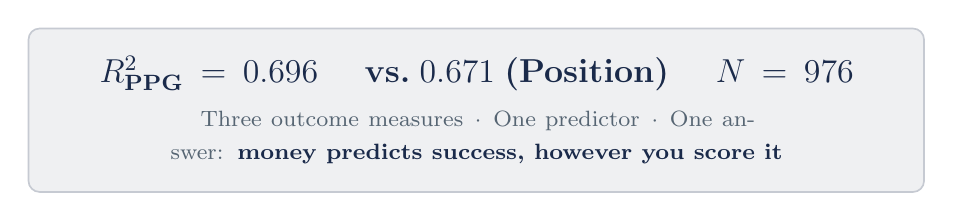
\begin{tikzpicture}
      \node[fill=NavyBlue!7, draw=NavyBlue!25, line width=0.6pt,
            rounded corners=4pt, inner sep=10pt,
            text width=0.88\linewidth, align=center]{%
        {\large\bfseries\color{NavyBlue}
          $R^2_{\text{PPG}} = 0.696$ \quad vs.\ $0.671$ (Position) \quad $N = 976$}\\[4pt]
        {\footnotesize\color{SlateGrey}
          Three outcome measures\enspace$\cdot$\enspace
          One predictor\enspace$\cdot$\enspace
          One answer: \textbf{\color{NavyBlue}money predicts success, however you score it}}
      };
    \end{tikzpicture}
  \end{center}
  \vspace{6pt}

  \begin{columns}[T]
    \begin{column}{0.48\textwidth}
      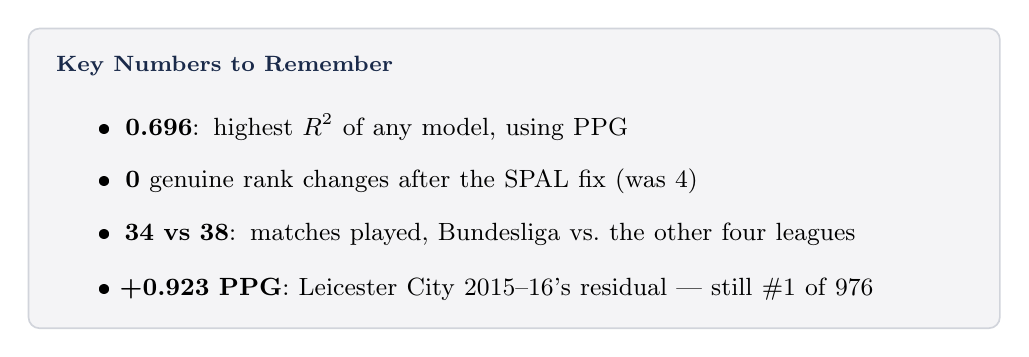
\begin{tikzpicture}
        \node[fill=NavyBlue!5, draw=NavyBlue!20, line width=0.6pt,
              rounded corners=4pt, inner sep=10pt,
              text width=\linewidth-14pt]{%
          {\footnotesize\bfseries\color{NavyBlue}Key Numbers to Remember}
          \vspace{4pt}
          \begin{itemize}\setlength\itemsep{4pt}
            {\small
            \item \textbf{0.696}: highest $R^2$ of any model, using PPG
            \item \textbf{0} genuine rank changes after the SPAL fix
                  (was 4)
            \item \textbf{34 vs 38}: matches played, Bundesliga
                  vs.\ the other four leagues
            \item \textbf{+0.923 PPG}: Leicester City 2015--16's
                  residual --- still \#1 of 976
            }
          \end{itemize}
        };
      \end{tikzpicture}
    \end{column}
    \begin{column}{0.48\textwidth}
      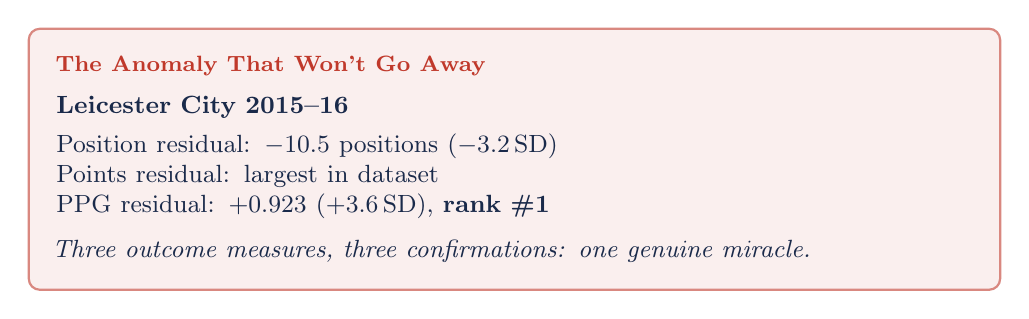
\begin{tikzpicture}
        \node[fill=AlertRed!8, draw=AlertRed!60, line width=0.8pt,
              rounded corners=4pt, inner sep=10pt,
              text width=\linewidth-14pt]{%
          {\footnotesize\bfseries\color{AlertRed}
            The Anomaly That Won't Go Away}\\[4pt]
          {\small\color{NavyBlue}
            \textbf{Leicester City 2015--16}\\[3pt]
            Position residual: $-10.5$ positions ($-3.2$\,SD)\\
            Points residual: largest in dataset\\
            PPG residual: $+0.923$ ($+3.6$\,SD), \textbf{rank \#1}\\[4pt]
            \textit{Three outcome measures, three confirmations:
            one genuine miracle.}}
        };
      \end{tikzpicture}
      \vspace{6pt}
      {\scriptsize\color{SlateGrey}
        \textbf{Data:} ESPN~FC + Transfermarkt (corrected)\quad
        \textbf{Period:} 2015--16 to 2024--25\\
        \textbf{Models:} OLS quadratic (Model H) across 3 outcome measures}
    \end{column}
  \end{columns}
\end{frame}

\end{document}
